\documentclass[cn,chinese,founder]{elegantbook}
\usepackage{wrapfig}
\everymath{\displaystyle}
% Useful commands:
% Add hyperlink:\href{http://example.com}{example}
%
% Adding wrapfig:
% \begin{wrapfigure}{r}{3.5cm}
%     \vspace{-1.5cm}
%     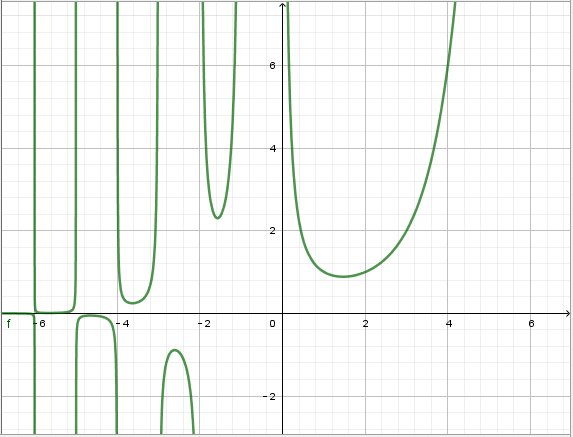
\includegraphics[width=3.5cm]{example.png}
%     \caption[示例]{示例解答图片}
% \end{wrapfigure}
% Please add it out of problem or solution envirnoment,or it behaves odd.

\begin{document}
\chapter{章节名}
 \section{节名}
  \subsection{思考题}
      \begin{example}
          在已证明下极限存在和$\varliminf_{n\to\infty}x_n=\lim_{n\to\infty}\inf_{k\geqslant n}\{x_k\}$成立的前提下利用$\varlimsup_{n\to\infty}x_n=-\varliminf_{n\to\infty}(-x_n)$来证明上极限存在和$\varlimsup_{n\to\infty}x_n=\lim_{n\to\infty}\sup_{k\geqslant n}\{x_k\}$成立.
      \end{example}
      \begin{solution}
          有公式$\varlimsup_{n\to\infty}x_n=-\varliminf_{n\to\infty}(-x_n)$和下极限存在之后上极限的存在就是简单推论.
      \end{solution}

  \subsection{练习题}
      \begin{exercise}
          求以下数列的上极限和下极限:
          \begin{enumerate}
              \item $x_n=\frac{1+(-1)^n}{2},n\in\mathbb{N}_+$;
                    \begin{solution}

                    \end{solution}
              \item $x_n=\sin\frac{n\pi}{4},n\in\mathbb{N}_+$;
              \item $x_n=n^{(-1)^n},n\in\mathbb{N}_+$;
              \item $x_n=e^{n(-1)^n},n\in\mathbb{N}_+$.
          \end{enumerate}
      \end{exercise}
\end{document}
